\documentclass[11pt, compress]{beamer}
\usepackage{amsmath}
\usetheme{Boadilla}
\usefonttheme[onlymath]{serif}
%get rid of navigation:
\setbeamertemplate{navigation symbols}{}


 %%%% Start PreTeXt generated preamble: %%%%% 

\newcommand{\tabularfont}{}
\usepackage[xparse, raster]{tcolorbox}
\tcbset{colback=white, colframe=white}
\NewTColorBox{image}{mmm}{boxrule=0.25pt, colframe=gray, left skip=#1\linewidth,width=#2\linewidth}
\RenewTColorBox{definition}{m}{colback=teal!30!white, colbacktitle=teal!30!white, coltitle=black, colframe=gray, boxrule=0.5pt, sharp corners=downhill, titlerule = 0.25pt, title={#1}}
\RenewTColorBox{theorem}{m}{colback=pink!30!white, colbacktitle=pink!30!white, coltitle=black, colframe=gray, boxrule=0.5pt, sharp corners=downhill, titlerule = 0.25pt, title={#1}}
\RenewTColorBox{proof}{}{boxrule=0.25pt, colframe=gray, colback=white, before upper={Proof:}, after upper={\qed}}
%% tcolorbox styles for sidebyside layout
\tcbset{ bwminimalstyle/.style={size=minimal, boxrule=-0.3pt, frame empty,
colback=white, colbacktitle=white, coltitle=black, opacityfill=0.0} }
\tcbset{ sbsstyle/.style={raster before skip=2.0ex, raster equal height=rows, raster force size=false} }
\tcbset{ sbspanelstyle/.style={bwminimalstyle} }
%% Enviroments for side-by-side and components
%% Necessary to use \NewTColorBox for boxes of the panels
%% "newfloat" environment to squash page-breaks within a single sidebyside
%% "xparse" environment for entire sidebyside
\NewDocumentEnvironment{sidebyside}{mmmm}
  {\begin{tcbraster}
    [sbsstyle,raster columns=#1,
    raster left skip=#2\linewidth,raster right skip=#3\linewidth,raster column skip=#4\linewidth]}
  {\end{tcbraster}}
%% "tcolorbox" environment for a panel of sidebyside
\NewTColorBox{sbspanel}{mO{top}}{sbspanelstyle,width=#1\linewidth,valign=#2}
%% For improved tables
\usepackage{array}
%% Some extra height on each row is desirable, especially with horizontal rules
%% Increment determined experimentally
\setlength{\extrarowheight}{0.2ex}
%% Define variable thickness horizontal rules, full and partial
%% Thicknesses are 0.03, 0.05, 0.08 in the  booktabs  package
\newcommand{\hrulethin}  {\noalign{\hrule height 0.04em}}
\newcommand{\hrulemedium}{\noalign{\hrule height 0.07em}}
\newcommand{\hrulethick} {\noalign{\hrule height 0.11em}}
%% We preserve a copy of the \setlength package before other
%% packages (extpfeil) get a chance to load packages that redefine it
\let\oldsetlength\setlength
\newlength{\Oldarrayrulewidth}
\newcommand{\crulethin}[1]%
{\noalign{\global\oldsetlength{\Oldarrayrulewidth}{\arrayrulewidth}}%
\noalign{\global\oldsetlength{\arrayrulewidth}{0.04em}}\cline{#1}%
\noalign{\global\oldsetlength{\arrayrulewidth}{\Oldarrayrulewidth}}}%
\newcommand{\crulemedium}[1]%
{\noalign{\global\oldsetlength{\Oldarrayrulewidth}{\arrayrulewidth}}%
\noalign{\global\oldsetlength{\arrayrulewidth}{0.07em}}\cline{#1}%
\noalign{\global\oldsetlength{\arrayrulewidth}{\Oldarrayrulewidth}}}
\newcommand{\crulethick}[1]%
{\noalign{\global\oldsetlength{\Oldarrayrulewidth}{\arrayrulewidth}}%
\noalign{\global\oldsetlength{\arrayrulewidth}{0.11em}}\cline{#1}%
\noalign{\global\oldsetlength{\arrayrulewidth}{\Oldarrayrulewidth}}}
%% Single letter column specifiers defined via array package
\newcolumntype{A}{!{\vrule width 0.04em}}
\newcolumntype{B}{!{\vrule width 0.07em}}
\newcolumntype{C}{!{\vrule width 0.11em}}
\newcommand{\terminology}[1]{\textbf{#1}}\newcommand{\lt}{<}
\newcommand{\gt}{>}
\newcommand{\amp}{&}


\renewcommand{\d}{\displaystyle}
\newcommand{\N}{\mathbb N}
\newcommand{\B}{\mathbf B}
\newcommand{\Z}{\mathbb Z}
\newcommand{\Q}{\mathbb Q}
\newcommand{\R}{\mathbb R}
\newcommand{\C}{\mathbb C}
\newcommand{\U}{\mathcal U}
\newcommand{\pow}{\mathcal P}
\newcommand{\inv}{^{-1}}
\newcommand{\st}{:}
\renewcommand{\iff}{\leftrightarrow}
\newcommand{\Iff}{\Leftrightarrow}
\newcommand{\imp}{\rightarrow}
\newcommand{\Imp}{\Rightarrow}
\newcommand{\isom}{\cong}

\renewcommand{\bar}{\overline}
\newcommand{\card}[1]{\left| #1 \right|}
\newcommand{\twoline}[2]{\begin{pmatrix}#1 \\ #2 \end{pmatrix}}

\newcommand{\vtx}[2]{node[fill,circle,inner sep=0pt, minimum size=4pt,label=#1:#2]{}}
\newcommand{\va}[1]{\vtx{above}{#1}}
\newcommand{\vb}[1]{\vtx{below}{#1}}
\newcommand{\vr}[1]{\vtx{right}{#1}}
\newcommand{\vl}[1]{\vtx{left}{#1}}
\renewcommand{\v}{\vtx{above}{}}

%% Graphics Preamble Entries
\usepackage{tikz, pgfplots}

\usetikzlibrary{positioning,matrix,arrows}

\usetikzlibrary{shapes,decorations,shadows,fadings,patterns}
\usetikzlibrary{decorations.markings}

\usepackage{skak} %for chessboards etc.

\def\circleA{(-.5,0) circle (1)}
\def\circleAlabel{(-1.5,.6) node[above]{$A$}}
\def\circleB{(.5,0) circle (1)}
\def\circleBlabel{(1.5,.6) node[above]{$B$}}
\def\circleC{(0,-1) circle (1)}
\def\circleClabel{(.5,-2) node[right]{$C$}}
\def\twosetbox{(-2,-1.4) rectangle (2,1.4)}
\def\threesetbox{(-2.5,-2.4) rectangle (2.5,1.4)}
\newcommand{\hexbox}[3]{
  \def\x{-cos{30}*\r*#1+cos{30}*#2*\r*2}
  \def\y{-\r*#1-sin{30}*\r*#1}
  \draw (\x,\y) +(90:\r) -- +(30:\r) -- +(-30:\r) -- +(-90:\r) -- +(-150:\r) -- +(150:\r) -- cycle;
  \draw (\x,\y) node{#3};
}

\tikzset{->-/.style={decoration={
  markings,
  mark=at position .5 with {\arrow{>}}},postaction={decorate}}}

  \newcommand{\onedot}{
    +(.5,.5) \v
  }
  \newcommand{\twodots}{
    +(.25,.25) \v +(.75,.75) \v
  }
  \newcommand{\threedots}{
  +(.25,.25) \v +(.5, .5) \v +(.75,.75) \v
  }
  \newcommand{\fourdots}{
    +(.25,.25) \v +(.25,.75) \v +(.75,.25) \v +(.75,.75) \v
  }
  \newcommand{\fivedots}{
    +(.5,.5) \v +(.25,.25) \v +(.25,.75) \v +(.75,.25) \v +(.75,.75) \v
  }
  \newcommand{\sixdots}{
    +(.25,.5) \v +(.75,.5) \v +(.25,.25) \v +(.25,.75) \v +(.75,.25) \v +(.75,.75) \v
  }
  \newcommand{\dominoborder}{
    \draw[thick, rounded corners] (0,0) rectangle (1,2);
    \draw[thin] (0,1) -- (1,1);
  }


%%%% End of PreTeXt generated preamble %%%%% 

\title{Functions}
\subtitle{(Section 0.4)}
\author{}
\date{}

\begin{document}
\begin{frame}
\maketitle 
\end{frame}
 
\begin{frame}
\frametitle{Overview}
\tableofcontents 
\end{frame}
 

\section{Definitions and Examples}
\begin{frame}
\frametitle{}
A \terminology{function} is a rule that assigns each input exactly one output. We call the output the \terminology{image} of the input. The set of all inputs for a function is called the \terminology{domain}. The set of all allowable outputs is called the \terminology{codomain}.
 
\pause \vfill 

We would write \(f:X \to Y\) to describe a function with name \(f\), domain \(X\) and codomain \(Y\). This does not tell us \emph{which} function \(f\) is though.
 
\pause \vfill 

To define the function, we must describe the rule. This is often done by giving a formula to compute the output for any input (although this is certainly not the only way to describe the rule).
\end{frame}
 
\begin{frame}
\frametitle{}
\begin{example}[0.4.1]The following are all examples of functions:
\pause 

\begin{enumerate}[<+->]
\item{} \(f:\Z \to \Z\) defined by \(f(n) = 3n\). The domain and codomain are all integers. The range is only the integer multiples of 3.


\item{} \(g: \{1,2,3\} \to \{a,b,c\}\) defined by \(g(1) = c\), \(g(2) = a\) and \(g(3) = a\). The domain is the set \(\{1,2,3\}\), the codomain is the set \(\{a,b,c\}\) and the range is the set \(\{a,c\}\). It is okay that \(g(2)\) and \(g(3)\) are the same element of the codomain: each element in the \emph{domain} still has only one output.


\item{} \(h:\{1,2,3,4\} \to \N\) defined by the table:
\begin{sidebyside}{1}{0}{0}{0}%
\begin{sbspanel}{1}%
{\centering%
{\tabularfont%
\begin{tabular}{lllll}
\multicolumn{1}{cA}{\(x\)}&1&2&3&4\tabularnewline\hrulethin
\multicolumn{1}{cA}{\(h(x)\)}&3&6&9&12
\end{tabular}
}%
\par}
\end{sbspanel}%
\end{sidebyside}%
Here the domain is the finite set \(\{1,2,3,4\}\) and to codomain is the set of natural numbers, \(\N\). This function is NOT the same as \(f\) defined above. Even though the rule is the same, the domain and codomain are different.

\end{enumerate}

\end{example}
\end{frame}
 
\begin{frame}
\frametitle{}
\begin{example}[0.4.2]Just because you can describe a rule in the same way you would write a function, does not mean that the rule is a function. The following are NOT functions.
\pause 

\begin{enumerate}[<+->]
\item{} \(f:\N \to \N\) defined by \(f(n) = \frac{n}{2}\). The reason this is not a function is because not every input has an output. Where does \(f\) send 3? The rule says that \(f(3) = \frac{3}{2}\), but \(\frac{3}{2}\) is not an element of the codomain.


\item{} Consider the rule that matches each person to their phone number. If you think of the set of people as the domain and the set of phone numbers as the codomain, then this is not a function, since some people have two phone numbers. Switching the domain and codomain sets doesn't help either, since some phone numbers belong to multiple people (assuming some households still have landlines when you are reading this).

\end{enumerate}

\end{example}
\end{frame}
 


\section{Describing Functions}
\begin{frame}
\frametitle{}
\begin{example}[0.4.3]Which of the following diagrams represent a function? Let \(X = \{1,2,3,4\}\) and \(Y = \{a,b,c,d\}\).
\begin{sidebyside}{3}{0.0416666666666667}{0.0416666666666667}{0.0833333333333333}%
\begin{sbspanel}{0.25}%
\resizebox{\linewidth}{!}{%
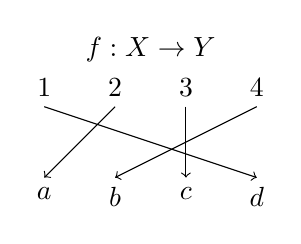
\begin{tikzpicture}[scale=0.9]
  \draw[->] (-1.5,1) node[above] {1} -- (1.5,0) node[below] {\(d\)};
  \draw[->] (-.5,1) node[above] {2} -- (-1.5,0) node[below] {\(a\)};
  \draw[->] (.5,1) node[above] {3} -- (.5, 0) node[below] {\(c\)};
  \draw[->] (1.5,1) node[above] {4} -- (-.5, 0) node[below] {\(b\)};
  \node[above] at (0,1.5) {$f:X \to Y$};
\end{tikzpicture}
}%
\end{sbspanel}%
\begin{sbspanel}{0.25}%
\resizebox{\linewidth}{!}{%
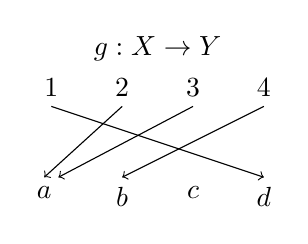
\begin{tikzpicture}[scale=0.9]
  \draw[->] (-1.5,1) node[above] {1} -- (1.5,0) node[below] {\(d\)};
  \draw[->] (-.5,1) node[above] {2} -- (-1.6,0) node[below] {\(a\)};
  \draw[->] (.5,1) node[above] {3} -- (-1.4, 0);
  \draw[->] (1.5,1) node[above] {4} -- (-.5, 0) node[below] {\(b\)};
  \draw (.5,0) node[below] {\(c\)};
  \node[above] at (0,1.5) { $g:X \to Y$};
\end{tikzpicture}
}%
\end{sbspanel}%
\begin{sbspanel}{0.25}%
\resizebox{\linewidth}{!}{%
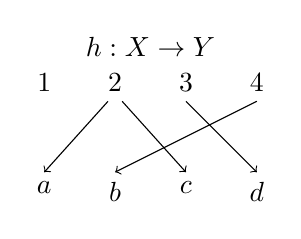
\begin{tikzpicture}[scale=0.9]
  \draw (-1.5,1) node[above] {1};
  \draw[->] (-.5,1) node[above] {2} (-.6,1) -- (-1.5,0) node[below] {\(a\)};
  \draw[->] (-.4,1) -- (.5,0);
  \draw[->] (.5,1) node[above] {3} -- (1.5, 0) node[below] {\(d\)};
  \draw[->] (1.5,1) node[above] {4} -- (-.5, 0) node[below] {\(b\)};
  \draw (.5,0) node[below] {\(c\)};
  \node[above] at (0,1.5) {$h:X \to Y$};
\end{tikzpicture}
}%
\end{sbspanel}%
\end{sidebyside}%
\end{example}
\end{frame}
 
\begin{frame}
\frametitle{Ways to describe functions}
 Here are three ways to describe the same function \(f:\{1,2,3\} \to \{1,2,3\}\):
 \begin{sidebyside}{2}{0.125}{0.125}{0.25}%
\begin{sbspanel}{0.25}%
\resizebox{\linewidth}{!}{%
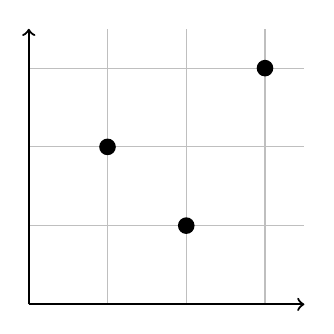
\begin{tikzpicture}[scale=1]
           \draw[thin, gray!50] (0,0) grid (3.5, 3.5);
           \draw[->, thick] (0,0) -- (0,3.5);
           \draw[->, thick] (0,0) -- (3.5,0);
           \fill (1,2) circle (3pt) (2,1) circle (3pt) (3,3) circle (3pt);
         \end{tikzpicture}
}%
\end{sbspanel}%
\begin{sbspanel}{0.25}%
\resizebox{\linewidth}{!}{%
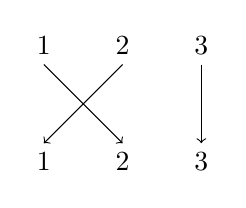
\begin{tikzpicture}[scale=1]
           \draw[->] (-1,1) node[above] {1} -- (0,0) node[below] {2};
           \draw[->] (0,1) node[above] {2} -- (-1,0) node[below] {1};
           \draw[->] (1,1) node[above] {3} -- (1,0) node[below] {3};
         \end{tikzpicture}
}%
\end{sbspanel}%
\end{sidebyside}%
 %
\begin{equation*}
f(x) = \begin{cases} x+1 \amp \text{ if } x = 1 \\ x-1 \amp \text{ if } x = 2 \\ x \amp \text{ if } x = 3\end{cases}\text{.}
\end{equation*}

\end{frame}
 
\begin{frame}
\frametitle{Tables and Two-Line Notation}
 For functions with small (finite) domains, defining the function through a table values is appropriate:
 \begin{sidebyside}{1}{0}{0}{0}%
\begin{sbspanel}{1}%
{\centering%
{\tabularfont%
\begin{tabular}{llllll}
\multicolumn{1}{cA}{\(x\)}&0&1&2&3&4\tabularnewline\hrulethin
\multicolumn{1}{cA}{\(f(x)\)}&3&3&2&4&1
\end{tabular}
}%
\par}
\end{sbspanel}%
\end{sidebyside}%
 
\pause \vfill 

We simplify this further by writing this as a ``matrix'' with each input directly over its output:%
\begin{equation*}
f = \twoline{0 \amp 1 \amp 2\amp 3 \amp 4}{3 \amp 3 \amp 2 \amp 4 \amp 1}\text{.}
\end{equation*}
Note this is just notation and not the same sort of matrix you would find in a linear algebra class (it does not make sense to do operations with these matrices, or row reduce them, for example).
\end{frame}
 
\begin{frame}
\frametitle{Closed and non-closed formulas}
 If the domain of a function is infinite (probably \(\N\) in this course), a \terminology{closed formula} might be a good way to describe the rule.  For example, \(f(n) = n^2\) is a closed formula.
 
\pause \vfill 

Compare that formula to the following, which is not a closed formula:
 \begin{example}[0.4.4]Consider the function \(f:\N \to \N\) given by \(f(0) = 0\) and \(f(n+1) = f(n) + 2n+1\). Find \(f(6)\).
\end{example}
\end{frame}
 
\begin{frame}
\frametitle{Recursively Defined Functions}
 For a function \(f:\N \to \N\), a \terminology{recursive definition} consists of an \terminology{initial condition} together with a \terminology{recurrence relation}. The initial condition is the explicitly given value of \(f(0)\). The recurrence relation is a formula for \(f(n+1)\) in terms for \(f(n)\) (and possibly \(n\) itself).
\end{frame}
 
\begin{frame}
\frametitle{}
\begin{example}[0.4.5]Give recursive definitions for the functions described below.
\pause 

\begin{enumerate}[<+->]
\item{} \(f:\N \to \N\) gives the number of snails in your terrarium \(n\) years after you built it, assuming you started with 3 snails and the number of snails doubles each year.


\item{} \(g:\N \to \N\) gives the number of push-ups you do \(n\) days after you started your push-ups challenge, assuming you could do 7 push-ups on day 0 and you can do 2 more push-ups each day.


\item{} \(h:\N \to \N\) defined by \(h(n) = n!\). Recall that \(n! = 1 \cdot 2 \cdot 3 \cdot \cdots \cdot (n-1)\cdot n\) is the product of all numbers from \(1\) through \(n\). We also define \(0! = 1\).

\end{enumerate}

\end{example}
\end{frame}
 


\section{Surjections, Injections, and Bijections}
\begin{frame}
\frametitle{Surjective functions}
 Sometimes there are elements of the codomain which are not in the range. When this sort of the thing \emph{does not} happen, (that is, when everything in the codomain is in the range) we say the function is \terminology{onto} or that the function maps the domain \emph{onto} the codomain.
 The fancy math term for an onto function is a \terminology{surjection}, and we say that an onto function is a \terminology{surjective} function.
 
\pause \vfill 

In pictures:
 \begin{sidebyside}{2}{0.1}{0.1}{0.2}%
\begin{sbspanel}{0.3}%
\resizebox{\linewidth}{!}{%
  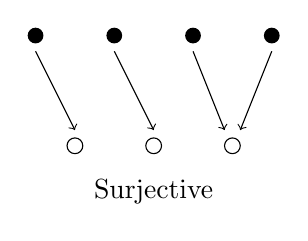
\begin{tikzpicture}
  \fill (-1.5, 1.2) circle (.1) (-.5,1.2) circle (.1) (.5, 1.2) circle (.1) (1.5,1.2) circle (.1);
  \draw[->] (-1.5, 1) -- (-1,0);
  \draw[->] (-.5,1) -- (0, 0);
  \draw[->] (.5, 1) -- (.9,0);
  \draw[->] (1.5,1) -- (1.1,0);
  \draw (-1, -0.2) circle (.1) (0, -0.2) circle (.1) (1, -0.2) circle (.1);
  \node[below] at (0,-.5) {Surjective};
\end{tikzpicture}
}%
\end{sbspanel}%
\begin{sbspanel}{0.3}%
\resizebox{\linewidth}{!}{%
  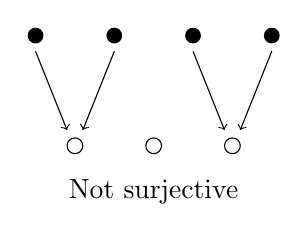
\begin{tikzpicture}
  \fill (-1.5, 1.2) circle (.1) (-.5,1.2) circle (.1) (.5, 1.2) circle (.1) (1.5,1.2) circle (.1);
  \draw[->] (-1.5, 1) -- (-1.1,0);
  \draw[->] (-.5,1) -- (-.9, 0);
  \draw[->] (.5, 1) -- (.9,0);
  \draw[->] (1.5,1) -- (1.1,0);
  \draw (-1, -0.2) circle (.1) (0, -0.2) circle (.1) (1, -0.2) circle (.1);
  \node[below] at (0,-.5) {Not surjective};
\end{tikzpicture}
}%
\end{sbspanel}%
\end{sidebyside}%
\end{frame}
 
\begin{frame}
\frametitle{}
\begin{example}[0.4.6]Which functions are surjective (i.e., onto)?\begin{enumerate}
\item{} \(f:\Z \to \Z\) defined by \(f(n) = 3n\).

\item{} \(g: \{1,2,3\} \to \{a,b,c\}\) defined by \(g = \begin{pmatrix}1 \amp 2 \amp 3 \\ c \amp a \amp a \end{pmatrix}\).

\item{} \(h:\{1,2,3\} \to \{1,2,3\}\) defined as follows:
\begin{sidebyside}{1}{0.4}{0.4}{0}%
\begin{sbspanel}{0.2}%
\resizebox{\linewidth}{!}{%
            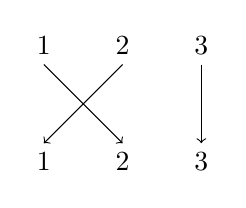
\begin{tikzpicture}
  \draw[->] (-1,1) node[above] {1} -- (0,0) node[below] {2};
  \draw[->] (0,1) node[above] {2} -- (-1,0) node[below] {1};
  \draw[->] (1,1) node[above] {3} -- (1,0) node[below] {3};
\end{tikzpicture}
}%
\end{sbspanel}%
\end{sidebyside}%

\end{enumerate}

\end{example}
\end{frame}
 
\begin{frame}
\frametitle{Injective functions}
 A function might assign the same element of the codomain to two or more different elements of the domain. When this \emph{does not} occur (that is, when each element of the codomain is the image of at most one element of the domain) then we say the function is \terminology{one-to-one}.
 The fancy math term for a one-to-one function is an \terminology{injection}. We call one-to-one functions \terminology{injective} functions.
 
\pause \vfill 

In pictures:
 \begin{sidebyside}{2}{0.05}{0.05}{0.1}%
\begin{sbspanel}{0.4}%
\resizebox{\linewidth}{!}{%
  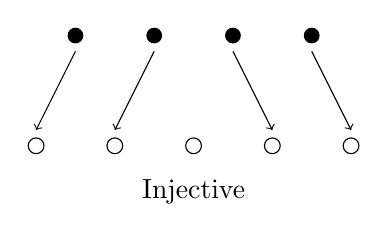
\begin{tikzpicture}
  \fill (-1.5, 1.2) circle (.1) (-.5,1.2) circle (.1) (.5, 1.2) circle (.1) (1.5,1.2) circle (.1);
  \draw[->] (-1.5, 1) -- (-2,0);
  \draw[->] (-.5,1) -- (-1, 0);
  \draw[->] (.5, 1) -- (1,0);
  \draw[->] (1.5,1) -- (2,0);
  \draw (-2, -0.2) circle (.1) (-1, -.2) circle (.1) (0, -0.2) circle (.1) (1, -0.2) circle (.1) (2, -0.2) circle (.1);
    \node[below] at (0,-.5) {Injective};
\end{tikzpicture}
}%
\end{sbspanel}%
\begin{sbspanel}{0.4}%
\resizebox{\linewidth}{!}{%
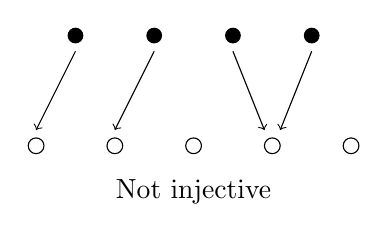
\begin{tikzpicture}
  \fill (-1.5, 1.2) circle (.1) (-.5,1.2) circle (.1) (.5, 1.2) circle (.1) (1.5,1.2) circle (.1);
  \draw[->] (-1.5, 1) -- (-2,0);
  \draw[->] (-.5,1) -- (-1, 0);
  \draw[->] (.5, 1) -- (.9,0);
  \draw[->] (1.5,1) -- (1.1,0);
  \draw (-2, -0.2) circle (.1) (-1, -.2) circle (.1) (0, -0.2) circle (.1) (1, -0.2) circle (.1) (2, -0.2) circle (.1);
    \node[below] at (0,-.5) {Not injective};
\end{tikzpicture}
}%
\end{sbspanel}%
\end{sidebyside}%
\end{frame}
 
\begin{frame}
\frametitle{}
\begin{example}[0.4.7]Which functions are injective (i.e., one-to-one)?\begin{enumerate}
\item{} \(f:\Z \to \Z\) defined by \(f(n) = 3n\).

\item{} \(g: \{1,2,3\} \to \{a,b,c\}\) defined by \(g = \begin{pmatrix}1 \amp 2 \amp 3 \\ c \amp a \amp a \end{pmatrix}\).

\item{} \(h:\{1,2,3\} \to \{1,2,3\}\) defined as follows:
\begin{sidebyside}{1}{0.4}{0.4}{0}%
\begin{sbspanel}{0.2}%
\resizebox{\linewidth}{!}{%
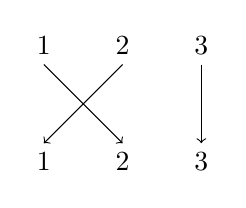
\begin{tikzpicture}
  \draw[->] (-1,1) node[above] {1} -- (0,0) node[below] {2};
  \draw[->] (0,1) node[above] {2} -- (-1,0) node[below] {1};
  \draw[->] (1,1) node[above] {3} -- (1,0) node[below] {3};
\end{tikzpicture}
}%
\end{sbspanel}%
\end{sidebyside}%

\end{enumerate}

\end{example}
\end{frame}
 
\begin{frame}
\frametitle{Injective vs Surjective}
 A function is \terminology{injective} provided every element of the codomain is the image of \emph{at most} one element from the domain.
 
\pause \vfill 

A function is \terminology{surjective} provided every element of the codomain is the image of \emph{at least} one element from the domain.
 
\pause \vfill 

A function might be both injective and surjective.  Such a functions is called a \terminology{bijection} (a \terminology{bijective function}).
\end{frame}
 


\section{Image and Inverse Image}
\begin{frame}
\frametitle{Images}
 The codomain element \(y\) that corresponds to a domain element \(x\) (that is, \(f(x) = y\)) is calle the \terminology{image} of \(x\).
 
\pause \vfill 

How can we describe the \emph{set} of images of elements from some subset of the domain? Suppose \(f:X \to Y\) is a function and that \(A \subseteq X\) is some subset of the domain (possibly all of it). We will use the notation \(f(A)\) to denote the \terminology{image of \(A\) under \(f\)}, namely the set of elements in \(Y\) that are the image of elements from \(A\). That is, \(f(A) = \{f(a) \in Y \st a \in A\}\).
\end{frame}
 
\begin{frame}
\frametitle{Inverse Image}
 We can do this in the other direction as well. We might ask which elements of the domain get mapped to a particular set in the codomain.
 
\pause \vfill 

Let \(f:X \to Y\) be a function and suppose \(B \subseteq Y\) is a subset of the codomain. Then we will write \(f\inv(B)\) for the \terminology{inverse image of \(B\) under \(f\)}, namely the set of elements in \(X\) whose image are elements in \(B\). In other words, \(f\inv(B) = \{x \in X \st f(x) \in B\}\).
 
\pause \vfill 

When \(B\) contains only one element, we write \(f\inv(y)\) instead of \(f\inv(\{y\})\).  But this is still a \emph{set}.
\end{frame}
 
\begin{frame}
\frametitle{}
\begin{example}[0.4.8]Consider the function \(f:\{1,2,3,4,5,6\} \to \{a,b,c,d\}\) given by%
\begin{equation*}
f = \begin{pmatrix}1 \amp 2 \amp 3 \amp 4 \amp 5 \amp 6 \\ a \amp a \amp b \amp b \amp b \amp c\end{pmatrix}\text{.}
\end{equation*}
Find \(f(\{1,2,3\})\), \(f\inv(\{a,b\})\), and \(f\inv(d)\).
\end{example}
\end{frame}
 
\begin{frame}
\frametitle{}
\begin{example}[0.4.9]Consider the function \(g:\Z \to \Z\) defined by \(g(n) = n^2 + 1\). Find \(g(1)\) and \(g(\{1\})\). Then find \(g\inv(1)\), \(g\inv(2)\), and \(g\inv(3)\).
\end{example}
\end{frame}
 
\begin{frame}
\frametitle{}
\begin{example}[0.4.10]Find a function \(f:\{1,2,3,4,5\} \to \N\) such that \(\card{f\inv(7)} = 5\).
\end{example}
\end{frame}
 

\end{document}
